\section{Results}

The simulation was conducted in GPGPU-Sim for NVIDIA Fermi GPU architecture \cite{bakhodayuan09}. GPGPU-Sim was configured to simulated the performance of GTX580, with all 16 streaming multiprocessors enabled (each CUDA streaming multiprocessor is represented as a single SIMT Core in GPGPU-Sim). Each streaming multiprocressor contains 48 warps, with 32 threads per warp (See Figure \ref{GTX580}). All sixteen SIMT cores share unified L2 cache.

\begin{figure}[ht!]
\centering
\label{GTX580}
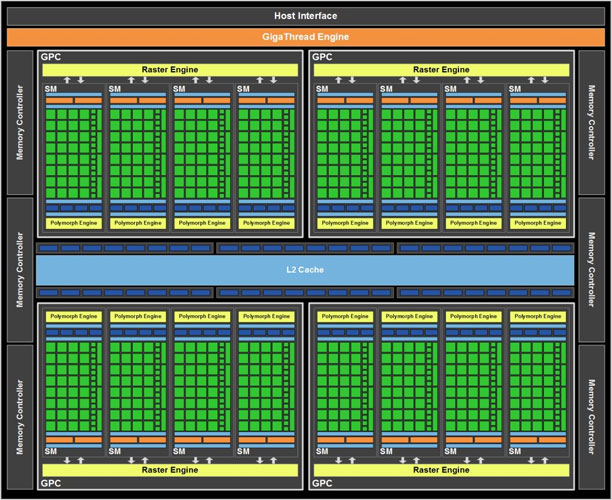
\includegraphics[width=90mm]{GTX580.jpg}
\caption{Block Diagram of Default GTX580. There are 16 SIMT Cores, all sharing a common L2 cache. Each SIMT Core contains a separate L1 cache.}
\end{figure}

In the original Fermi architecture, each streaming multiprocessor has its own distinct L1 cache. Each L1 instruction cache is a 4-way set associative, with 4 sets of 128 bytes blocks. To assess the  performance of different L1 instruction cache architecture, only the L1 instruction cache was modified, while all other variables remained constant. Other aspects of the architecture such as the bandwidth of shared L2 cache could serve as a performance bottleneck for different cache designs. However, these variables are assumed to have little impact on the hit and stall rate of the instruction cache, which are the primary metrics of interest.

The simulation results of are expected to show two optimization approaches in improving instruction cache performance by sharing multiple GPU cores share the cache. One approach is to keep the total instruction cache size constant and improve the performance of the cache, as shown in Figure \ref{HitImprov}. In this approach, when multiple cores are configured to share the same instruction cache, the previous cache that existed with each core are merged together to form larger caches. The increased sized of the cache may result in degredation in access time, but improves the hit rate. The hit rate of the cache is expected to improve greatly when the size of initial cache is doubled or tripled, but there will be less improvement when the hit rate at a high level.

\begin{figure}[t]
\centering
\label{HitImprov}
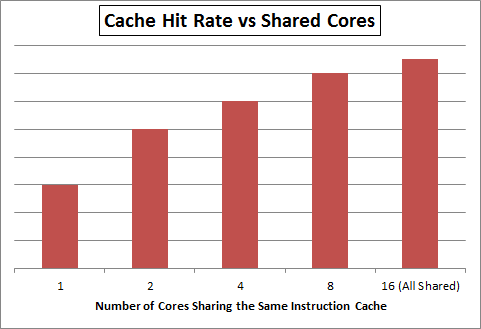
\includegraphics[width=90mm]{HitRateImprov.png}
\caption{Projected Improvement in Hit Rate. Total size of the instruction cache remains constant. Size of individual instruction cache is scaled proportionally to the number of cores that share the cache.}
\end{figure}


\begin{figure}[b!]
\centering
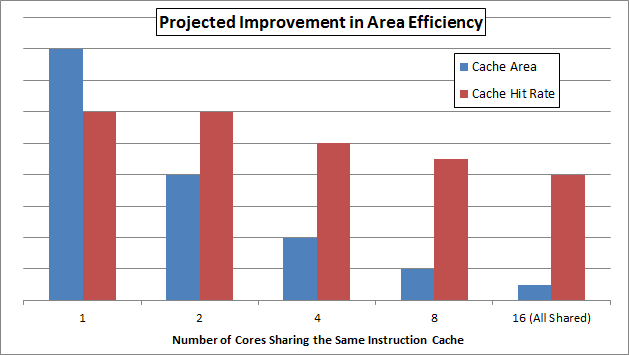
\includegraphics[width=90mm]{AreaEff.png}
\caption{Projected Improvement in Area Efficiency. Size of individual instruction cache remains constant, while the number of cores sharing the L1 cache is increased. The instruction redundancy between the cores should allow cache hit rate to remain high as cache area is reduced. }
\label{AreaEff}
\end{figure}


The second approach is to reduce the total size of the cache by keeping the size of individual instruction cache constant. In this approach, rather than merging the shared caches together, the instruction caches are kept at the same size even if more cores are sharing the same core. The hit rate of the cache may drop when the instruction cache is not large enough to satisfy all the cores sharing the cache, but this drop in hit rate is expected to be less than the reduction in area due to the instruction redundancy between the shared cores.


\subsection{Benchmarks}
Describe benchmarks used \jbs{Akhil in charge.}
Several benchmark programs were used in this project. These benchmarks included STO, RAY, NQU, LPS, LIB, CP and BFS. In order to determine which of the aforementioned benchmarks would be most useful for the purposes of our project, we performed an experiment in which the performance of the benchmarks was examined as a function of the number of cores used in the available GTX580 architecture. The number of cores was varied between 1 and 16 (the maximum number of cores available on the GTX580). Then the miss and stall rate was noted for each different architectural configuration. Figure \ref{fig:missStalls} shows the results of our experiment. 

\begin{figure}[b!]
\centering
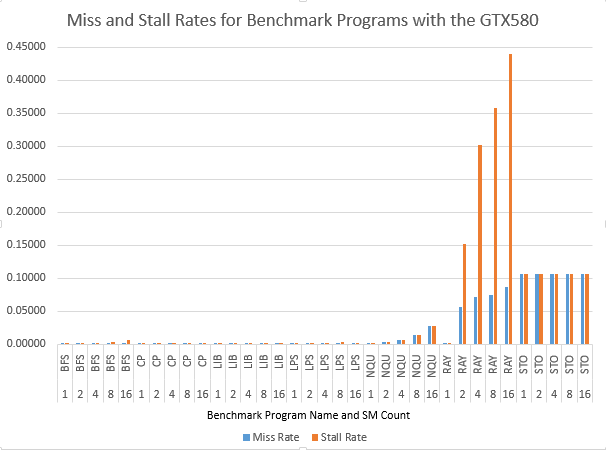
\includegraphics[width=90mm]{miss_stalls_benchmarks.png}
\caption{Miss and Stall Rates for Benchmark Programs with the GTX580}
\label{fig:missStalls}
\end{figure}

\begin{figure}[b!]
\centering
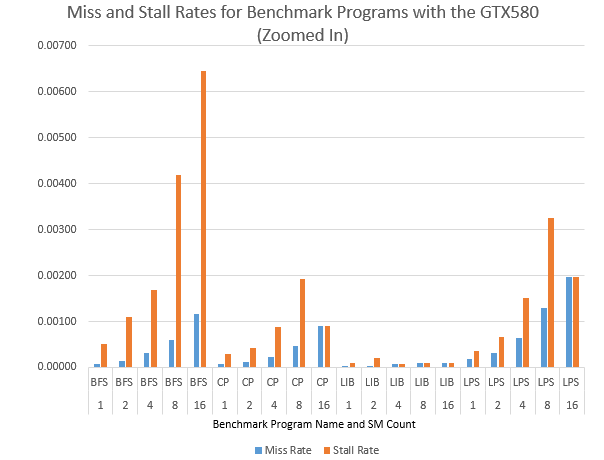
\includegraphics[width=90mm]{miss_stalls_benchmarks_zoomed.png}
\caption{Miss and Stall Rates for Benchmark Programs with GTX580 (Zoomed In) }
\label{fig:missStallsZoomed}
\end{figure}

Figure \ref{fig:missStallsZoomed} is a zoomed in version of \ref{fig:missStalls} included to enable better understanding of the results with lower miss rates. 

The benchmark STO is hardly affected by this and RAY has a much higher stall rate (indicating more reservation fails than misses) than its miss rates, and is relatively very affected. RAY did have a bit more variability in how it was affected by the core numbers.

In order to explain the reasons behind the results shown in Figures \ref{fig:missStalls} and \ref{fig:missStallsZoomed}, we examined the degree of parallelism of RAY and CP.

The degree of parallism is a representation of the number of software work elements that each program issues to the GPU when executing in hardware. The following calculations have been derived from the CUDA source files and are a representation of the level of parallelism employed by 2 programs which we found interesting as per our previous results. \\

\emph{RAY}\\

Number of threads in each block $= 16 \times 8 = 128$ threads

Number of thread blocks $= (64/16, 64/8) = (4,8)$

Thus, number of thread blocks in a queue at any given time $= 4 \times 8 = 32.$
\\

\emph{Coulombic Potential (CP)}\\

Number of threads in each block $= 16 \times 8 = 128$ threads.

VOLSIZEX $= 512$

VOLSIZEY $= 512$

BLOCKSIZEX $= 16$

BLOCKSIZEY $= 8$

UNROLLX  $= 1$

Grid Size in the x dimension $= Gsz.x = 512/16 = 32$

Grid Size in the y dimension $= Gsz.y = 512/8 = 64$

Grid Size in the z dimension $=$ UNROLLX $= 1$

Thus the number of thread blocks issued $= (32, 64)$

and the number of blocks in the queue at a given point in time $= 32 \times 64 = 2048$ thread blocks.

The reason only the parallelism of CP and RAY were examined was that from a preliminary inspection, they seemed to having a desired combination of parallelism and size of instruction set. 

From all the aforementioned results, it was clear that RAY was the most interesting bechmark. This was because it had the highest number of PTX instructions issued and was also significatly parallel. Moreover, the fact that the degree of parallelism of RAY could be increased easily by modifying the CUDA program, we nominated RAY as our most significant benchmark program. 

Increasing the degree of parallelism in software entailed changing the image size that the Ray Tracer would operate on and the number of thread blocks (and consequently the number of threads in the queue at a given time). The following are the calculations related to the tweaked version of RAY which serves as an indicator of the degree of parallelism with which RAY executes on the GPU:

Number of threads in each block $= 16 x 8 = 128$ threads

Number of thread blocks issued $= (512/16, 512/8) = (32, 64)$

Thus the number of blocks in the queue at a given time $= 32 x 64 = 2048.$

This ensured that the RAY benchmark was executing as parallel in software as the Coulombic Potential benchmark in the number of work elements that it was issuing. Given that the RAY CUDA file issues more instructions in its core computation that CP does, and that a lot of its instructions (CUDA instructions) seem to be computationally more expensive, RAY can now be treated as both a long program which would occupy a significant amount of space in the instruction cache (and hence would not be entirely resident in the instruction cache) AND would issue those instructions with a high degree of parallelism.

\subsection{Preliminary Results}
\jbs{Fabiha in charge}

